\section{Proposed Methodology} \label{scene}
This section gives a detailed description of our proposed approach for action recognition in video. The methodology in this paper follows the conventional action recognition pipeline. Given a set of labelled videos, a set of features is extracted from each video, represented using visual descriptors, and combined into a single video descriptor, which is used to train a multi-class classifier for recognition. \B{It will be easier to have a pipeline image that shows the different stages of processing: (1) extract dense improved trajectories, (2) foreground/background trajectory separation, (3) compute descriptors for the foreground (BoF on MBH, HOF, etc for each trajectory), the camera motion (BoF on frame-to-frame estimated fundamental matrices), and the context (BoF on the background appearance).}

In this paper, we use dense point trajectories (short tracks of a densely sampled set of pixels in a video \cite{wang2013}) as our primitive features. By estimating frame-to-frame camera motion (fundamental matrix), we separate foreground trajectories corresponding to the action from background ones. Each type of trajectory is represented using a different descriptor. Foreground trajectories are represented using conventional visual properties (e.g. MBH, HOF, HOG, and trajectory shape), while the background appearance is described using SIFT. Foreground and background trajectories are then encoded separately using the BoF framework. Unlike other action recognition methods, we not only use the frame-to-frame camera motion to separate foreground from background, but we also use it to \emph{describe} a video. This is done by encoding all frame-to-frame fundamental matrices in a video using the BoF framework. We use all three descriptors (foreground, background/context, and camera motion) to train a multi-class classifier for recognition. \B{Let's move most of the implementation details from the experiments to here.} In this paper, we argue and show that combining a foreground-only description \cite{wang2013} with additional cues (background/context and camera motion) provides a richer and more discriminative description of actions.

\B{Since camera motion is used in the foreground-background separation part too, I recommend we move the the camera motion subsection to be first, then the  separation subsection, then the context/background subsection}


%describes our methodology for capturing background information or \textit{contextual features}. We present a novel approach for including description of background trajectories. We argue that combining a pure foreground description \cite{wang2013} with additional surrounding cues have a significant contribution to action description. To obtain these background trajectories, we perform a weak foreground-background separation based on the trajectory displacement. Then, we explicitly model the global motion in the video and the context appearance using those background feature points.




\subsection{Foreground-Background Separation}
In order to recover foreground action only information, we need to separate the extracted dense trajectories into foreground or background. Some information related to the actor are included on the Improved Trajectories approach. It results beneficial when capturing the spatio-temporal appearance of human actions. However, we claim that modeling contextual information needs to be performed on background feature points. \B{Fabian, the previous three sentences need to be rephrased and expanded for clarity. I didnt quite understand what you meant here.} We apply a simple strategy to weakly label trajectory features. We compute trajectories as described in \cite{wang2013}, but also compute the sum of the Frobenius norm for the displacement vector as follows:

\begin{equation}
D = \sum _{j=t}^{t+L-1}\left ( (x_{t+1}-x_t)^2, (y_{t+1}-y_t)^2 \right ),
\end{equation}

This measure allow us to perform a binary trajectory segmentation: (a) if $D>\alpha$ trajectory is labeled as foreground and (b) for $D<=\alpha$ correspond a background trajectory. Empirically, we set this threshold value to $\alpha=3$ pixels. \B{There is no mention of using camera motion compensation here? Fabian, please elaborate more here.}

In Figure \ref{fig:approach}, we show the results of applying our weak trajectory separation on three sample video sequences. Here, foreground and background trajectories are colored coded in red and blue respectively. Clearly, the foreground trajectories correspond to the underlying action itself, while background trajectories correspond to \emph{static} background pixels undergoing camera motion only. Our proposed separation will allow each type of trajectory (foreground and background) to be represented independently and thus more reliably than other methods that encode context information using all features \cite{marszalek2009}.


\begin{figure*}[t!]
\begin{center}
%\fbox{\rule{0pt}{3in} \rule{0.9\linewidth}{0pt}}
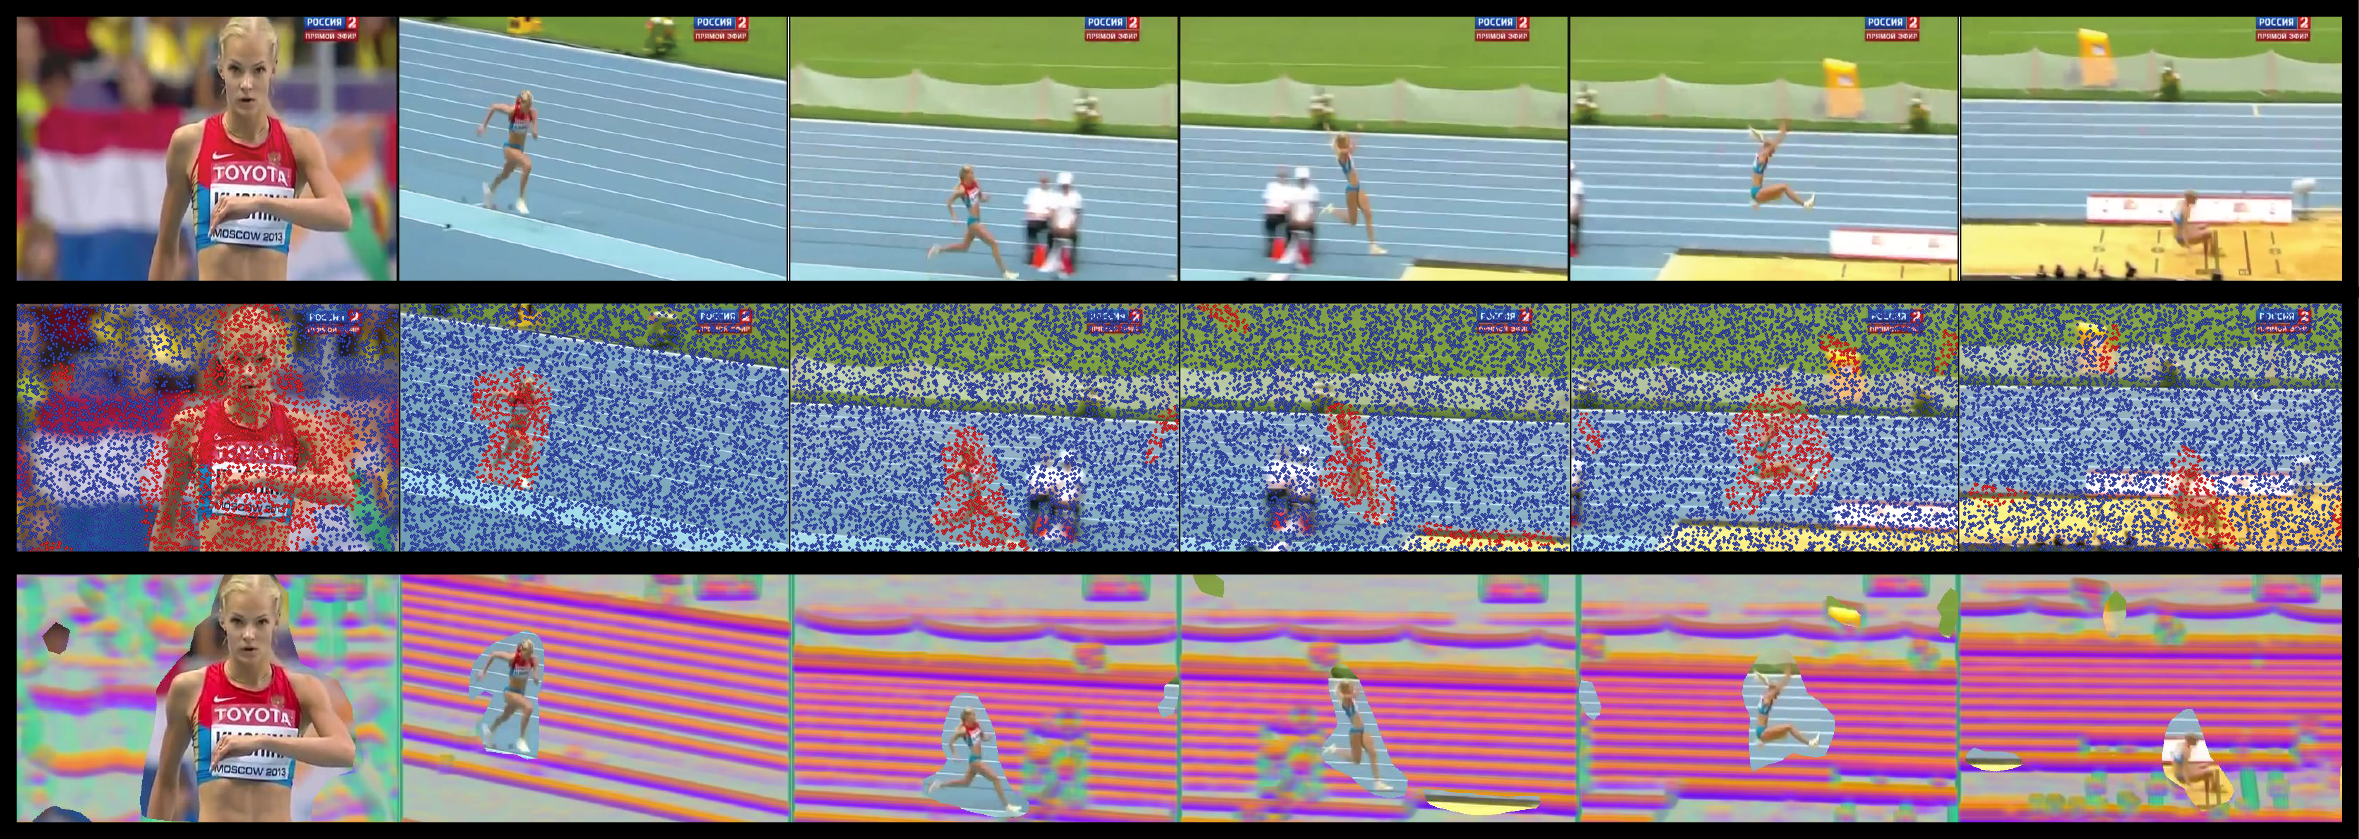
\includegraphics[width=0.98\linewidth]{fig/approach.png}
\end{center}
\caption{Overview of our method. \textbf{Top}. Frame sequence sampled from a long jump video. Note that the video contains a translation movement following the subject. \textbf{Middle}. Camera compensation allows to perform a background-foreground segmentation. Noticeably, foreground feature points are mostly related with the subject. \textbf{Bottom}. Illustration of captured information by SIFT. In order to achieve a meaningful illustration, descriptor dimensionality is reduced to 3 dimensions and output within a color code image. As illustrated, contextual appearance is captured only from pixels related with the scenario \ie avoiding pixels related with the subject with execute the action.}
\label{fig:approach}
\end{figure*}


\subsection{Generic Camera Motion}
Since videos are normally filmed with the intention of maintaining the subject within the image frame, there exists a relationship between the estimated camera motion and the underlying action. In this paper, we argue and show that this relationship can be a useful cue for discriminating certain action classes. \B{We need some visual examples here of actions where this comment is true.}. Here, we do not claim that this cue is significant for all types of actions, since very similar camera motion can be shared among classes. \B{We need an example here about action classes where camera motion wont help discrimination.} Instead of using a homography to encode camera motion, we estimate the more general fundamental matrix for each pair of frames in a video using the well-known 8-point algorithm \cite{eightpoint97}. As mentioned earlier, a homography is suitable to describe camera motion when the camera is not translating or when the background is planar; however, it is not applicable in more complex or cluttered scenes.

After estimating all pairwise fundamental matrices, we encode the camera motion of a video using the BoF framework. This descriptor complements other visual descriptors of the video. Unlike most existing work, we embrace camera motion and employ a low-level feature to capture this global motion in the video.


\subsection{Background/Context Appearance}
Human actions could be recognized by a set of cues. Beyond local motion and appearance properties of an action, the context in which an action is performed is a critical component to recognize actions. For example, a 'springboard' action can only be executed if there is a pool, which has distinctive appearance properties. This motivates us to encode the visual appearance of the static scene. Background/context appearance is encoded using SIFT descriptors \cite{lowe2004} around trajectory points associated with the background. We detect SIFT keypoints in a dense manner and then filter out those that fall within the union of foreground trajectories. Context appearance focuses more on the scenario itself, as observed in Figure \ref{fig:approach}. \B{elaborate on this example and the relationship to context} Unlike other methods that encode context holistically in a video \cite{marszalek2009}, separating the background/context from the foreground produces a more reliable and robust context descriptor.

\begin{figure*}[t!]
\begin{center}
%\fbox{\rule{0pt}{3in} \rule{0.9\linewidth}{0pt}}
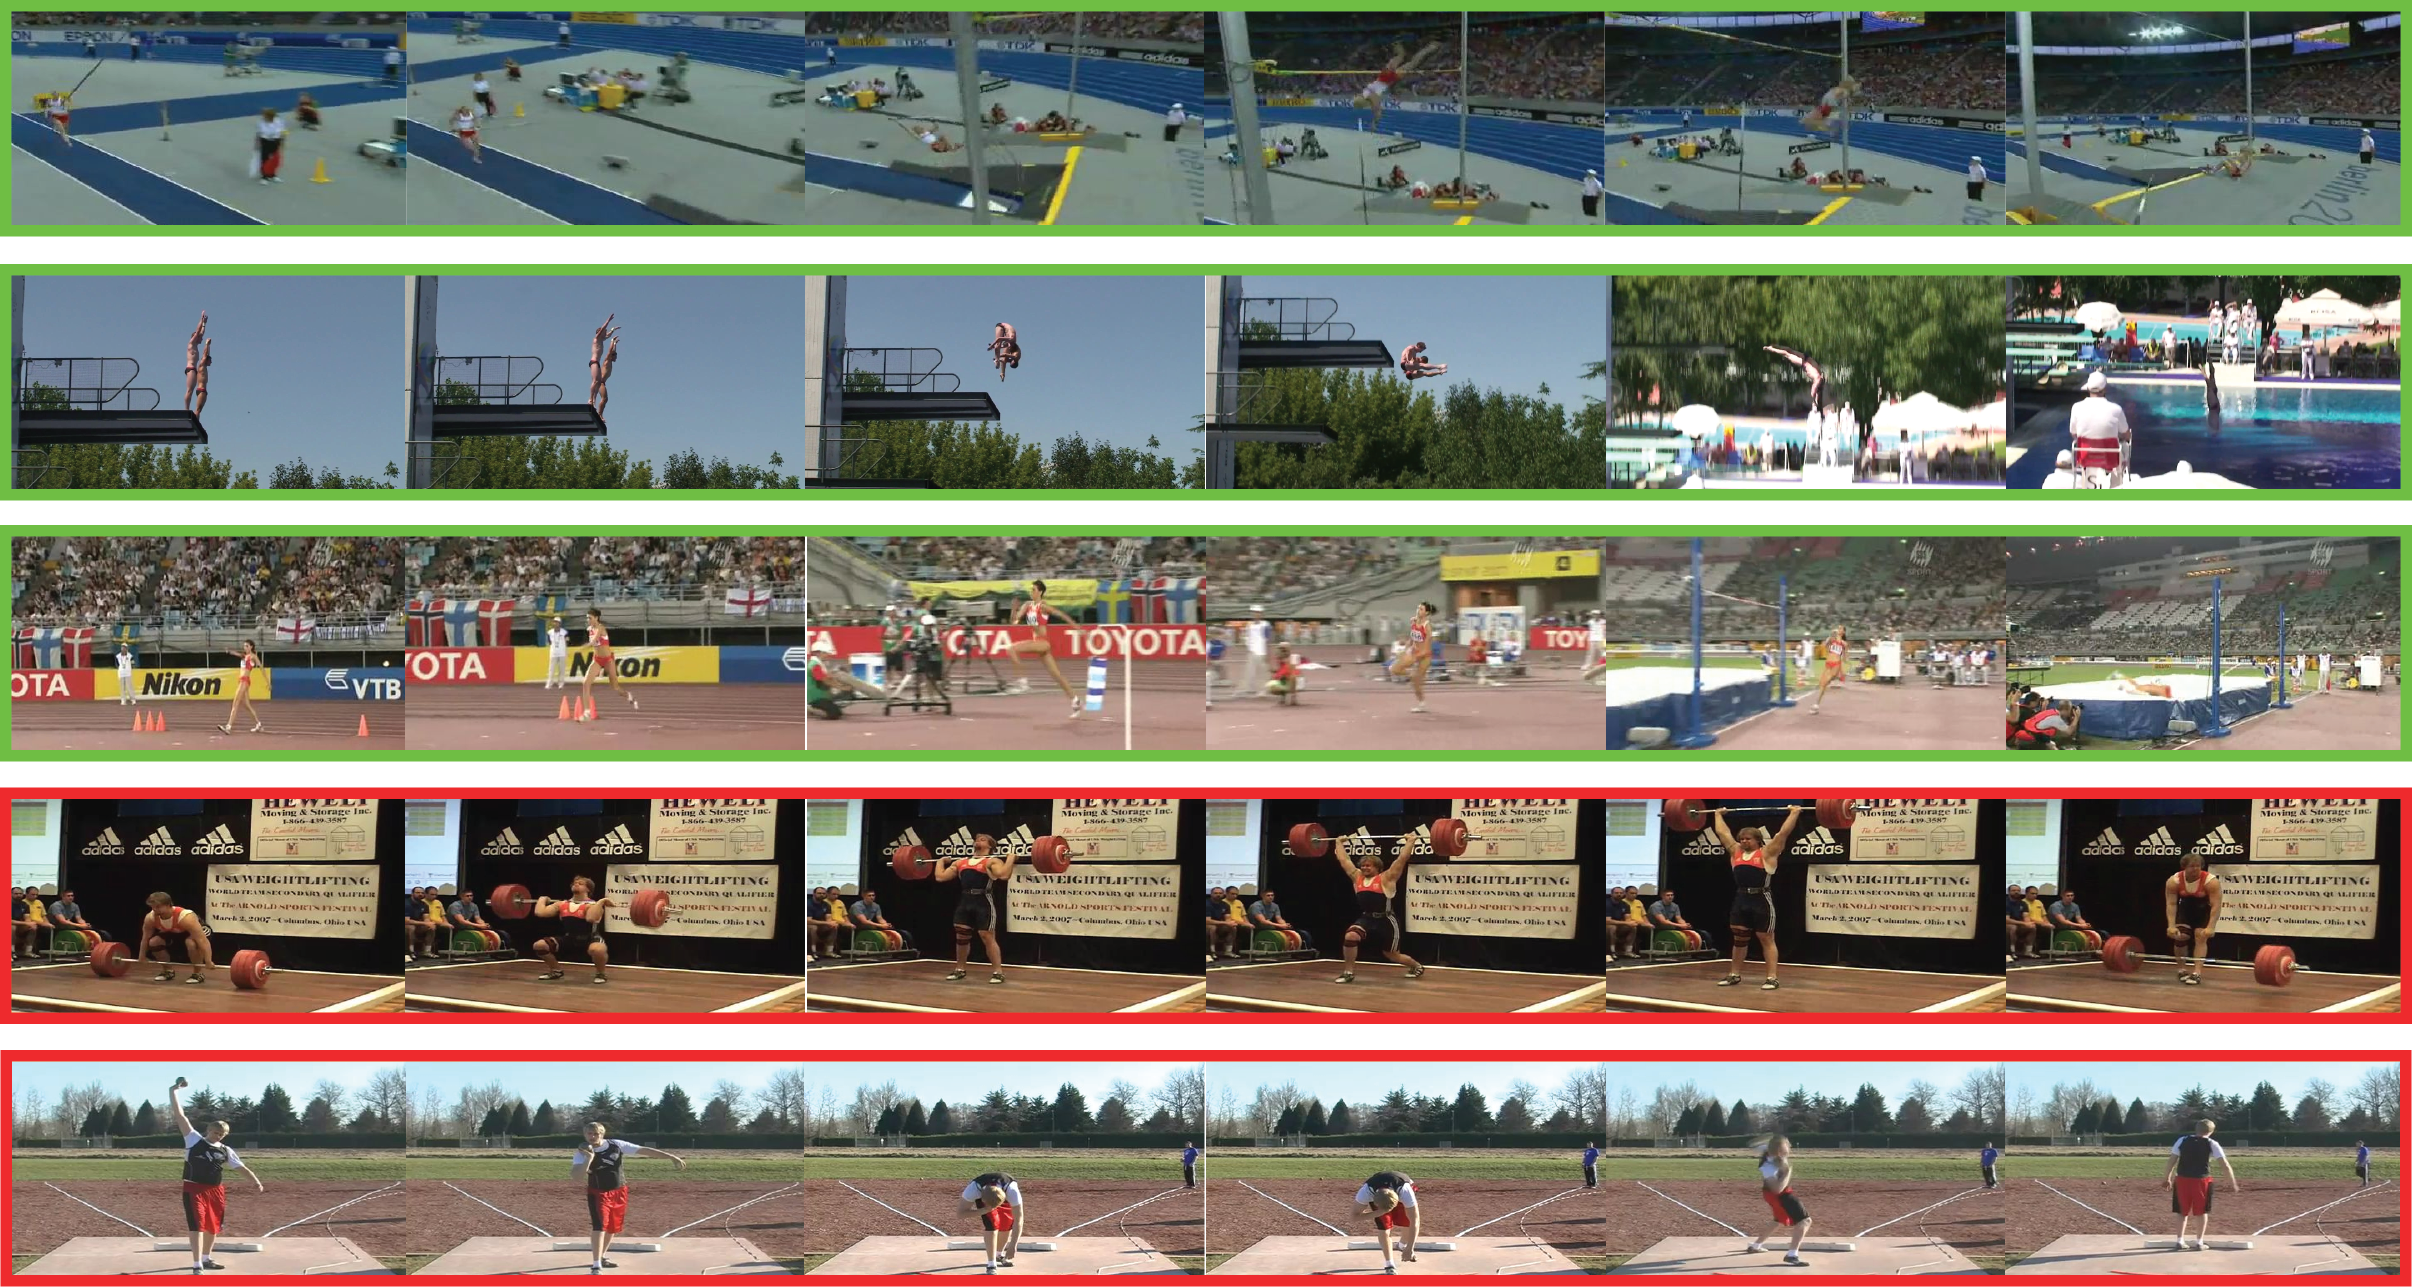
\includegraphics[width=0.98\linewidth]{fig/camMotion.png}
\end{center}
\caption{A generic camera motion descriptor can be a useful cue for discriminating specific action categories. As illustrated, the three first rows contains a characteristic correlation between how camera moves and the associated action. Unfortunately, this type of cue its not significant for all type of actions as shown in the last two rows where camera not move at all.}
\label{fig:camMotion_example}
\end{figure*}

\begin{figure*}[t!]
\begin{center}
%\fbox{\rule{0pt}{3in} \rule{0.9\linewidth}{0pt}}
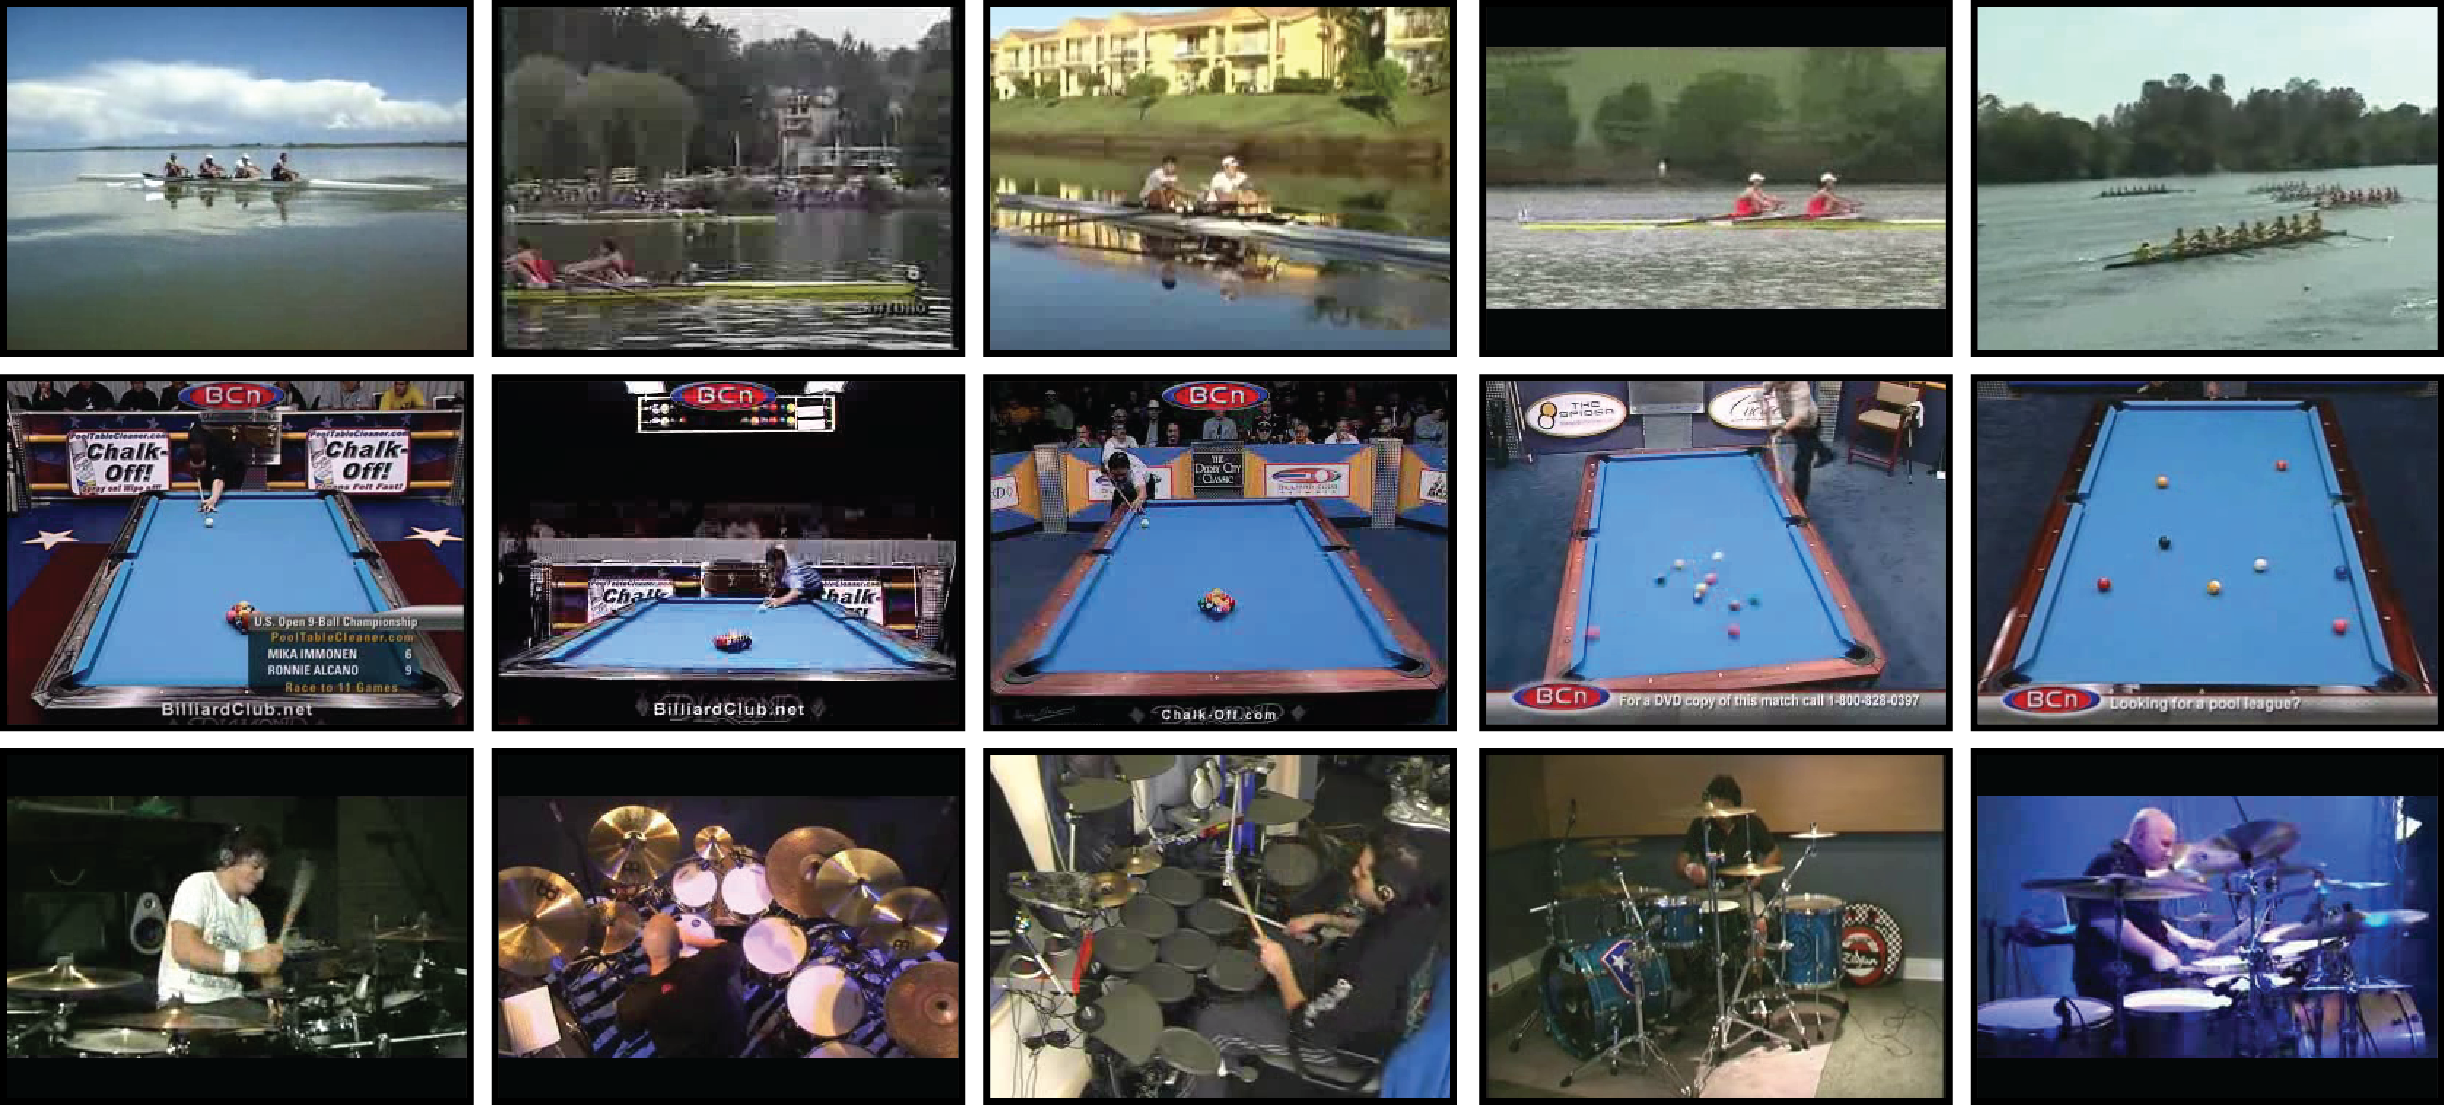
\includegraphics[width=0.98\linewidth]{fig/sift.png}
\end{center}
\caption{Each row presents five different thumbnails taken from different videos of UCF50 dataset. \textbf{Top} row corresponds to rowing's examples. As observed all thumbnails share distinct background appearance \ie in all water is present and also in the majority there is a common landmark. In the \textbf{Middle} row, different billiard examples are depicted. Billard table and also the indoor naturalness of the action, enables context appearance to capture critical information about the action. Finally, \textbf{Bottom} row exposes examples from the drumming category. As noticed, all of the examples share a lot of visual cues that mostly are avoided if only foreground features are used.}
\label{fig:sift_example}
\end{figure*}